\documentclass{acm_proc_article-sp}

\usepackage[T1]{fontenc}
\usepackage{polyglossia}
\setdefaultlanguage{english}
\usepackage{csquotes}

\usepackage{fontspec}
\usepackage{xltxtra}
\usepackage{libertine}

\usepackage[usenames, dvipsnames]{xcolor}
\graphicspath{{./img/}}

\usepackage[backend=biber, style=alphabetic]{biblatex}
\bibliography{literatur.bib}

\usepackage{subcaption}
\usepackage{fancyref}

\usepackage[%
unicode=true,%
colorlinks=true,%
linkcolor=black,%
urlcolor=MidnightBlue,%
citecolor=black,%
filecolor=black%
]
{hyperref}


\newcommand{\todo}[1]{\textcolor{Red}{#1}}
\newcommand{\sebastian}[1]{\textcolor{Green}{#1}}
\newcommand{\stefan}[1]{\textcolor{BurntOrange}{#1}}
\newcommand{\etal}{\textit{et. al.}}

\begin{document}

\title{
Interactive Simulation WS 15/16\\ %
Project Proposal
}
\subtitle{EYES - Exchange Your Vision Simulator}
\numberofauthors{2}
\author{
% 1st. author
\alignauthor
Sebastian Lemp\\
%       \affaddr{Street, House}\\
%       \affaddr{PLZ City}\\
%       \affaddr{Country}\\
%       \email{sebastian.lemp@student.uni-augsburg.de}
% 2nd. author
\alignauthor
Stefan Büttner\\
%       \affaddr{Street, House}\\
%       \affaddr{PLZ City}\\
%       \affaddr{Country}\\
%       \email{stefan.buettner@student.uni-augsburg.de}
}
%\additionalauthors{Additional Authors}

% The date is actually not used in the acm template
\date{University of Augsburg, \today}

% Not neede for our purposes
%\terms{Terms}
%\keywords{Keyword 1, Keyword 2}
%% A category with the (minimum) three required fields
%\category{H.4}{Information Systems Applications}{Miscellaneous}
%%A category including the fourth, optional field follows...
%\category{D.2.8}{Software Engineering}{Metrics}[complexity measures, performance measures]

%% For the ACM ToG format
%\acmformat{ACMFormat}
%\acmVolume{Vol.}
%\acmNumber{Nr.}
%\acmYear{YYYY}
%\acmMonth{MM}
%\acmArticleNum{XXX}
%\doi{DOI}


\maketitle
%\begin{abstract}
%\end{abstract}

% Disease list:
% -------------------------------------------------------------------------------
% (Stefan)     11 Disorders of sclera, cornea, iris and ciliary body
% (Sebastian)   1 Cataract (Grauer Star)
% (Stefan)      2 Retinal detachment and breaks
% (Sebastian)  14 Other retinal disorders
% (Stefan)      1 Glaucoma (Grüner Star)
% (Stefan)      2 Disorders of optic nerve and visual pathways
% (Sebastian)  10 Disorders of ocular muscles, binocular movement, accommodation and refraction
% (Stefan)      6 Visual disturbances and blindness
%              47

%
% Possible References:
% http://www.svi.cps.utexas.edu/EI466209.pdf

% http://www.icdvrat.org/2008/papers/ICDVRAT2008_S04_N06_Banks_McCrindle.pdf
%
% claim they have an real-time app for Android and iOS:
% http://www.brailleinstitute.org/sight-loss-blog/398-leading-eye-diseases.html 
%
% OpenGL real-time simulation
% http://percept.eecs.yorku.ca/papers/p127-vinnikov.pdf
% 

\section{Motivation}
Eye diseases have been an issue throughout all the human history. In the
beginning the focus layed on their treatment. This task is reasonably well
solved for many diseases and since Virtual Reality (VR) is more and more
pushing into the consumer market, it could be broardly used for education and
thus prevention of eye diseases. For example, the risk of suffering from
retinal detachment can be greatly reduced if the signs are recognized early
and a doctor is consulted. Therfore, educational software can be used.
In addition, people would hopefully visit a doctor earlier if they already
experienced a good simulation of a severe state of a disease, before they
actually are in a severe state.
Other applications could be testing designs of consumer products like packaging
or traffic signs or other signs at public places.

Altough there are many simulations available already, they usually work on
still 2D images, 2D video streams or static 3D scenes\footnote{All these
statements are based on our brief research. There might still be game-like
applications out there... somewhere.} and don't have any game component.
Moreover, more sophisticated simulations are probably not easily available
for public use and implementing a simulator using Unity3D in terms of an
\emph{eye disease asset set} wrapped into a small game could be interesting
for a broard audience.

%\begin{itemize}
%  \item Give people the opportunity to experience different symptoms of eye
%      disease, to know what they are and how to fight them for example
%      nightblindness can caused by a wrong diet
%      ⇒ so help people to eat the right food.
%  \item Supposedly there is already a real-time simulator for eye diseases for
%      Android, although we were not able to find it on Google Play Store for
%      our phones \cite{braille}.
%\end{itemize}

\section{Concept}
%\begin{itemize}
%  \item Fulfill everyday tasks with impaired vision
%  \item Possible boni: 
%  \begin{itemize}
%    \item Get rid of disease by performing the right actions
%    e.g. take medication on the way or make a doctors appointment...
%    \item Preventive measures during the task to not get disease in next lvl
%  \end{itemize}
%  \item Target platform: Android \& Google Cardboard to address many people
%\end{itemize}

The user should be able to experience different types of eye diseases,
including early as well as severe stages in order to understand when to consult
a doctor and why. Hopefully, this gives people better judgement on when to
visit a doctor as well as the courage to do so, if they experience the symptoms
of a particular disease.

There will be at least the first 6 different eye diseases in
\Fref{tab:eye_diseases} either to choose from in every task or appear at least
once in the game.

Possible tasks could be based on reading (visual acuity), distinguishing
objects (color), and navigating in everyday environments
(limited field of view).
This may be realized required for cooking, working at a line in a factory
sorting screws or similar things, using public transport or driving a car
(at night), food shopping, going to the pharmacy getting the right medication,
find hidden object given written hints, or board/care games.

Ideally the chosen tasks would be individual levels which depend on eachother
and will tell a small story, like cardriving → food shopping → cooking.
The user can either choose the disease for the level himself or a random disease
is selected in the beginning.
The chosen disease should become worse over the time (within one level or
across levels) but, if possible and accurate (neglecting the time), the user
should also be able to slow down the process or even heal the disease
completely. Therefore he/she has to take the appropriate measures for the
specific disease.

\section{Project Requirements}
Vinnikov \etal \cite{gazedisplays} developed a Gaze-Contingent-Display in order
to evaluate the users eye direction and adept the displayed images in real-time.
Because the effects of eye diseases follow the eye movement, i.e. are static
with respect to the eye coordinate frame, they achieved more realistic results
in comparison to rendering gaze-independant images.

However the german company SensoMotoric Instruments (SIM) provides an gaze
tracking solution update for the Oculus Rift DK 2 \cite{smi-oculus, arstechoculus}.
Like the Oculus, it's
still under development but could probably already be purchased. There is also
an integration into various VR engines, including Unity3D available making it
especially interesting for this project.

The gaze-direction would be useful to accurately simulate the vision field
and would also be an interesting human interface for the game mechanics.

\begin{figure}
    \centering
    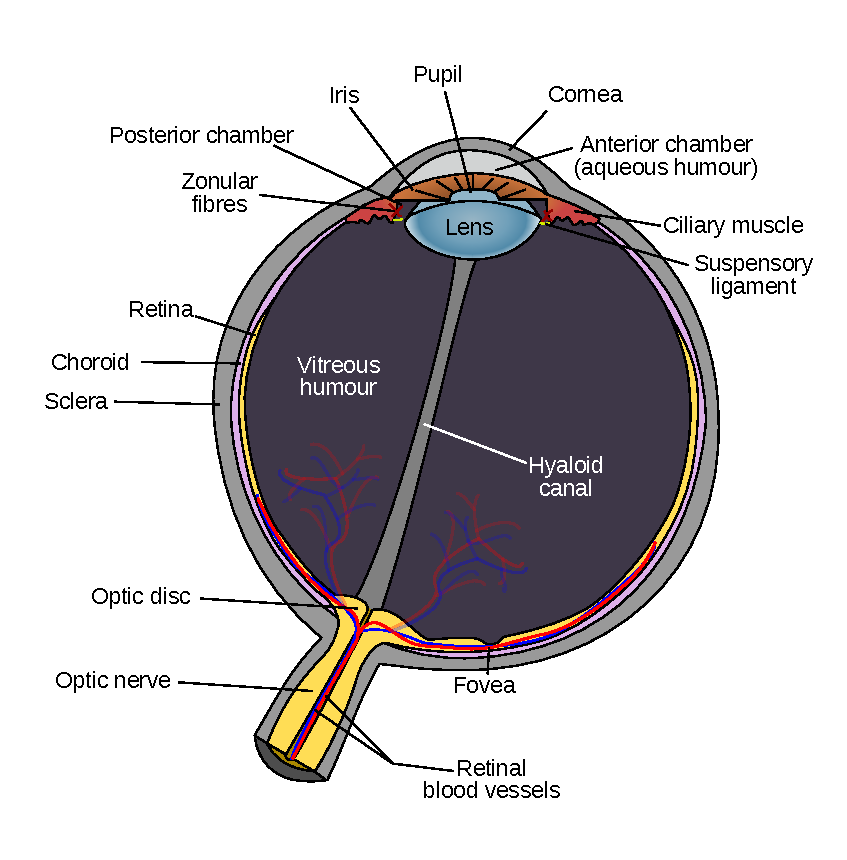
\includegraphics[width=\columnwidth]{human_eye_scheme.pdf}
    \caption{Scheme of the human eye.}
    \label{humaneye}
\end{figure}

\begin{table}
    \textbf{Glaucoma}\\
    Sudden eye pain, blurred vision and loss of vision espacilly in the
    outer regions.

    \vspace{1em}\textbf{Cataracts}\\
    Blurred vision especially in the center region.

    \vspace{1em}\textbf{Diabetic Retinopathy}\\
    Black spots in the view.

    \vspace{1em}\textbf{Color blindness}\\
    Some colours appear undistinguishable.

    \vspace{1em}\textbf{Achromatopsia}\\
    (Almost) No color sensitivity at all.

    \vspace{1em}\textbf{Myopia / Hyperopia}\\
    Commonly known as nearsightness and farsightness respectively.

    \vspace{1em}\textbf{Kreatoconus}\\
    The cornea deforms into a conical shape.
    Multiple ghost images may be visible, arranged in a chaotic pattern,
    the vision becomes blurry, and visual acuity decreases at all distances.
    Poor night vision, photophobia, and eye strain are additional symptoms.

    \vspace{1em}\textbf{Nyctalopia / Hermalopia}\\
    High difficulty to see in relatively low and bright light respectively.

    \vspace{1em}\textbf{Retinal detachment / Posterior viterous detachment}\\
    Flashes of light, very brief in the extreme peripheral region.
    Sudden increase in the amount of floaters.
    Slight feeling of heaviness in the eye.
    \caption{Eye diseases}
    \label{tab:eye_diseases}
\end{table}

\section{Timeline}

\begin{itemize}

  \item Research

  \begin{itemize}

    \item What kind of eye diseases are most common?
	
    \item Are there Simulators like this available?
	
    \item Find some suitable task.

    \item How to implement custom camera projections in Unity?

    \item How to interface with the oculus rift?

        
  \end{itemize}

  \item Implementation

  \begin{itemize}

    \item Create scenario/level 1

    \item Implement the first disease

    \item Implement the other diseases 

    \item Create another scenario

    \item Create menu

    \item Integrate oculus rift

  \end{itemize}

  \item Testing
  
  \item Presentation and Report

\end{itemize}




\todo{}
\printbibliography

\balancecolumns

\end{document}
